% VUT FIT MITAI
% MSZ 2021/2022
% Author: Vladimir Dusek
% Login: xdusek27

%%%%%%%%%%%%%%%%%%%%%%%%%%%%%%%%%%%%%%%%%%%%%%%%%%%%%%%%%%%%%%%%%%%%%%%%%%%%%%%%

% Path to figures
\graphicspath{{pdi/volba_koordinatora}}

%%%%%%%%%%%%%%%%%%%%%%%%%%%%%%%%%%%%%%%%%%%%%%%%%%%%%%%%%%%%%%%%%%%%%%%%%%%%%%%%

\chapter{Klasifikace algoritmů volby koordinátora, algoritmus Bully a jeho složitost.}

%%%%%%%%%%%%%%%%%%%%%%%%%%%%%%%%%%%%%%%%%%%%%%%%%%%%%%%%%%%%%%%%%%%%%%%%%%%%%%%%

\section{Metadata}

\begin{compactitem}
    \item Předmět: Prostředí distribuovaných aplikací (PDI)
    \item Přednáška:
    \begin{compactitem}
        \item 7) Synchronizace
    \end{compactitem}
    \item Záznam:
    \begin{compactitem}
        \item 2020-11-02
    \end{compactitem}
\end{compactitem}

%%%%%%%%%%%%%%%%%%%%%%%%%%%%%%%%%%%%%%%%%%%%%%%%%%%%%%%%%%%%%%%%%%%%%%%%%%%%%%%%

\section{Úvod a kontext}

\begin{compactitem}
    \item Mějme množinu procesů v~rámci distribuovaného systému. Řešíme problém  nalezení shody na nějaké věci (synchronizační problém). Problém můžeme rozdělit na dvě situace:
    \begin{compactitem}
        \item \textbf{Problém volby koordinátora} -- Výběr jednoho z~procesů, který bude vedoucím procesem (koordinátor). Tento proces pak může vykonat určitou činnost nebo může sloužit ostatním procesům k~realizaci  význačné role v~systému.
        \item \textbf{Problém vzájemného vyloučení} -- Předpokládejme, že konkrétní zdroj může v~daném okamžiku používat pouze jeden proces. Tento problém se běžně vyskytuje ve víceprocesorových systémech, ale také v~distribuovaných systémech.
    \end{compactitem}
    \item Synchronizační problémy lze v~rámci operačních systémů nebo multiprocesorových systémů řešit pomocí provádění atomických operací, sdílené paměti apod. (je pro ně podpora v~rámci operačního systému nebo hardwaru). V~distribuovaných systémech nic takového není z~principu možné a proto se synchronizační problémy řeší pomocí zasílání zprav, resp. algoritmicky.
\end{compactitem}

%%%%%%%%%%%%%%%%%%%%%%%%%%%%%%%%%%%%%%%%%%%%%%%%%%%%%%%%%%%%%%%%%%%%%%%%%%%%%%%%

\section{Problém volby koordinátora}

\begin{compactitem}
    \item Předpokládáme:
    \begin{compactitem}
        \item Každý proces má unikátní ID.
        \item Procesy neznají stav (běžící, neběžící) dalších procesů.
        \item Každý proces zná ID dalších procesů (záleží na topologii).
    \end{compactitem}
    \item Cíl:
    \begin{compactitem}
        \item Dosáhnutí shody mezi všemi procesy na procesu, který je koordinátor.
        \item Kritérium výběru koordinátora může být různé. Např. na základě proces ID (proces s~největším ID se stane koordinátorem).
    \end{compactitem}
\end{compactitem}

%%%%%%%%%%%%%%%%%%%%%%%%%%%%%%%%%%%%%%%%%%%%%%%%%%%%%%%%%%%%%%%%%%%%%%%%%%%%%%%%

\section{Bully algoritmus}

Pro topologii každý s~každým -- každý proces může komunikovat s~každým dalším procesem. Používá tři druhy zpráv: ELECTION, OK, COORDINATOR.

\subsection{Postup}

\begin{compactitem}
    \item Proces P, který má podezření, že chybí koordinátor, může zahájit volby.
    \begin{compactenum}
        \item Proces P odešle zprávu ELECTION všem procesům s~větším ID.
        \item Pokud nikdo neodpoví, P vyhrává volby a stává se koordinátorem.
        \item Pokud některý z~procesů s~větším ID odpoví (zpráva OK), tak přebírá řízení a práce P je ukončena.
        \item Pokud P obdrží zprávu ELECTION od procesů s~menším ID, pošle jim odpověď OK na zablokování procesů.
    \end{compactenum}
    \item Nakonec zůstane pouze P (nový koordinátor), který o~tom informuje ostatní zasláním zprávy COORDINATOR.
    \item Pokud se proces probudí nebo je restartován, první akcí je vyvolání voleb.
\end{compactitem}

\subsection{Složitost}

Složitost z~hlediska počtu zpráv.

\bigskip\noindent Nejhorší případ (iniciátor s~nejmenším ID):

\begin{compactitem}
    \item $(n-1)$ iterací
    \item $2(n-1)$ zpráv ELECTION a OK pro každou iteraci
    \item $(n-1)$ zpráv COORDINATOR
    \item Celkem: $(n-1) \times 2(n-1) + (n-1) \approx n^2$
\end{compactitem}

\noindent Nejlepší případ (iniciátor s~největším ID):

\begin{compactitem}
    \item $(n-1)$ zpráv COORDINATOR
    \item Celkem: $(n-1)$
\end{compactitem}

\subsection{Příklad}

\begin{figure}[H]
    \centering
    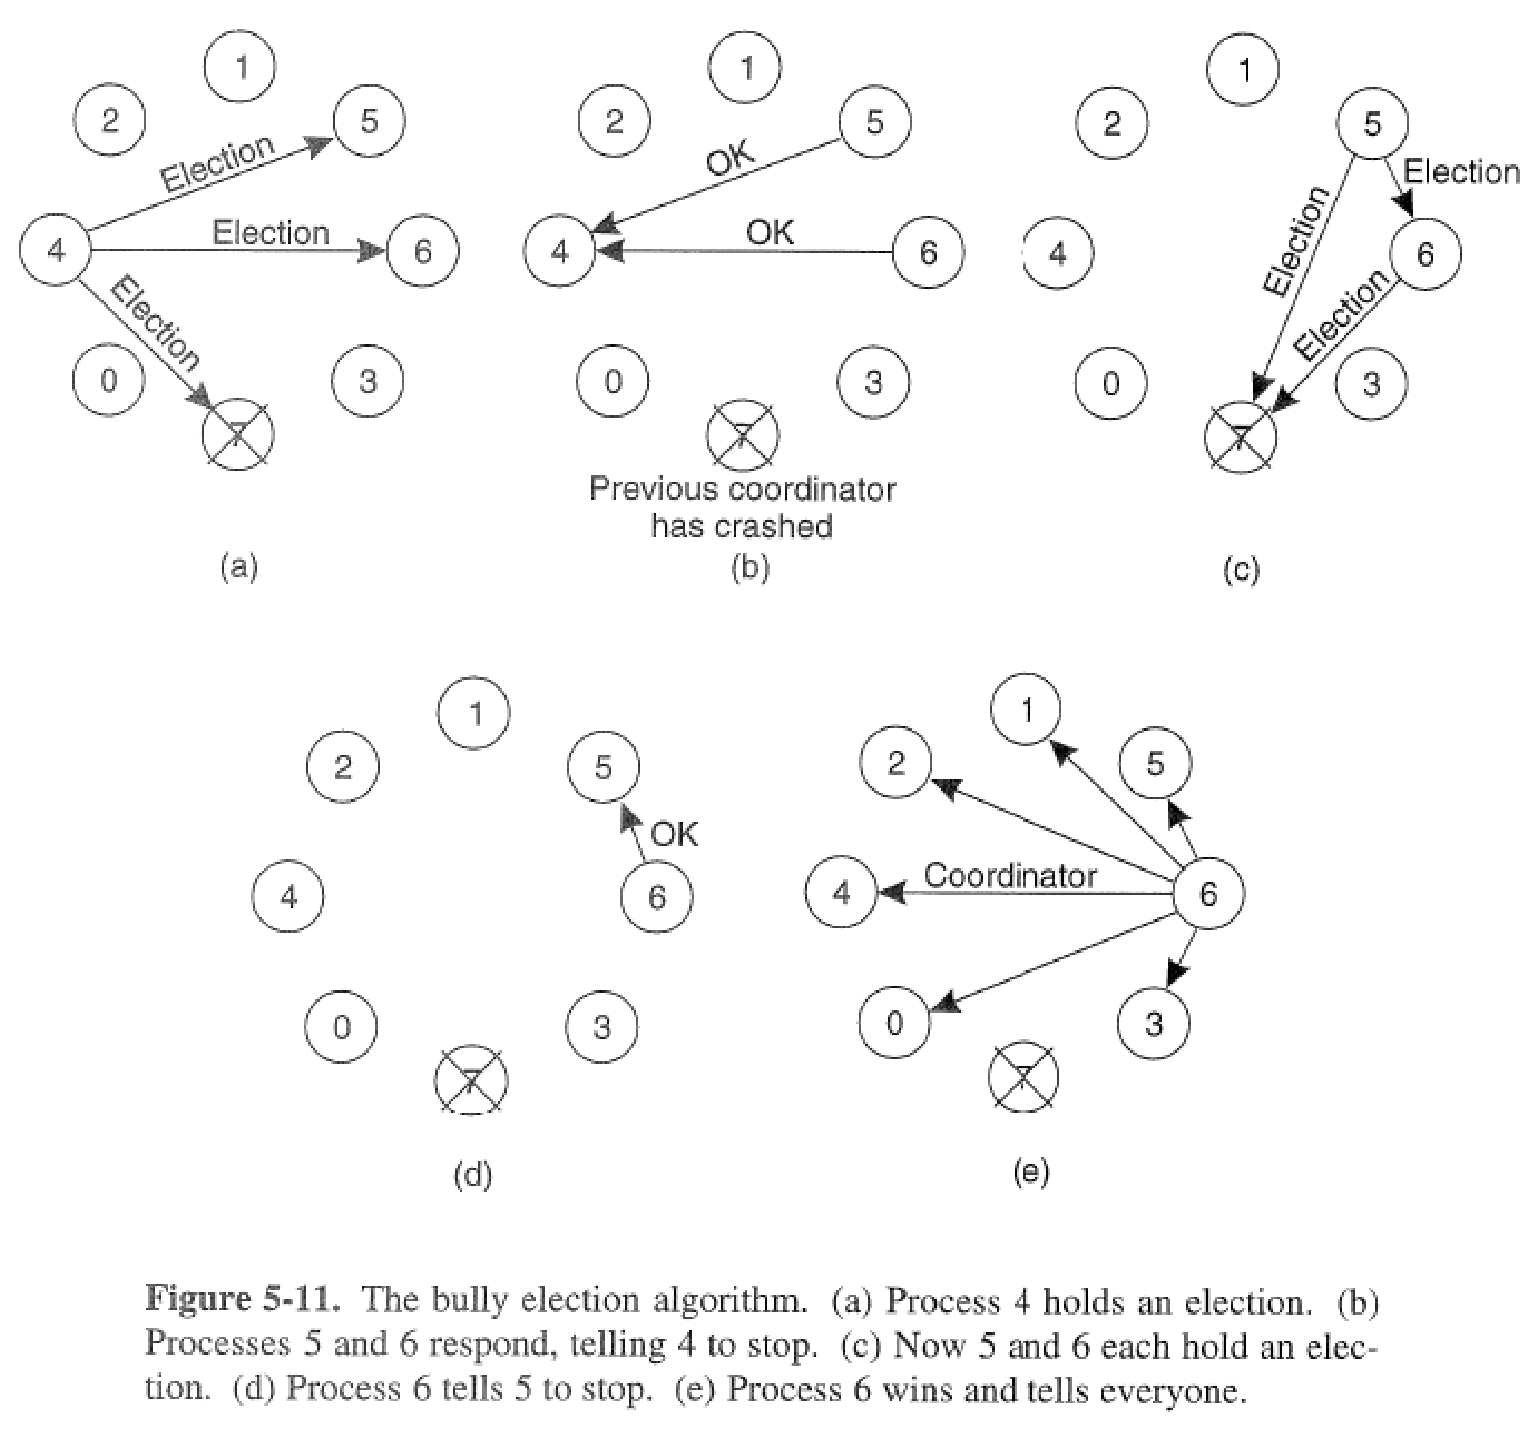
\includegraphics[width=1\linewidth]{example_bully.pdf}
    \caption{Příklad činnosti Bully algoritmu.}
\end{figure}

%%%%%%%%%%%%%%%%%%%%%%%%%%%%%%%%%%%%%%%%%%%%%%%%%%%%%%%%%%%%%%%%%%%%%%%%%%%%%%%%

\section{Ring Algoritmus}

Pro kruhovou topologii -- procesy jsou uspořádané do kruhu podle svého proces ID.
Každý proces musí vědět nejenom o~svém následovníkovi, ale také o~jeho následníkovi, který funguje jako \uv{záloha}, v~případě že by se přímý následník stal nedostupný. Používá dva druhy zpráv: ELECTION, COORDINATOR.

\subsection{Postup}

\begin{compactitem}
    \item Proces P, který má podezření, že chybí koordinátor, může zahájit volby.
    \begin{compactenum}
        \item Zašle zprávu ELECTION obsahující jeho ID dalšímu procesu (pokud další proces nereaguje, proces P zašle stejnou zprávu dalšímu v~kruhu).
        \item Každý člen topologie přijme zprávu ELECTION, přidá do ní své ID a přepošle zprávu dalšímu procesu.
    \end{compactenum}
    \item Když se zpráva vrátí k~procesu P, je zpráva převedena na zprávu  COORDINATOR a poslána následujícímu procesu v~topologii, aby bylo možné nahlásit:
    \begin{compactenum}
        \item Novým koordinátorem se stává proces s~nejvyšším ID.
        \item Členové sítě jsou stále aktivní.
    \end{compactenum}
    \item Po síti může obíhat více zpráv zároveň.
\end{compactitem}

\subsection{Složitost}

Složitost z~hlediska počtu zpráv.

\bigskip\noindent Vždy $2n \approx n$ zpráv. Jedno kolečko \uv{oběhne} zpráva ELECTION a druhé zpráva COORDINATOR.

\subsection{Příklad}

\begin{figure}[H]
    \centering
    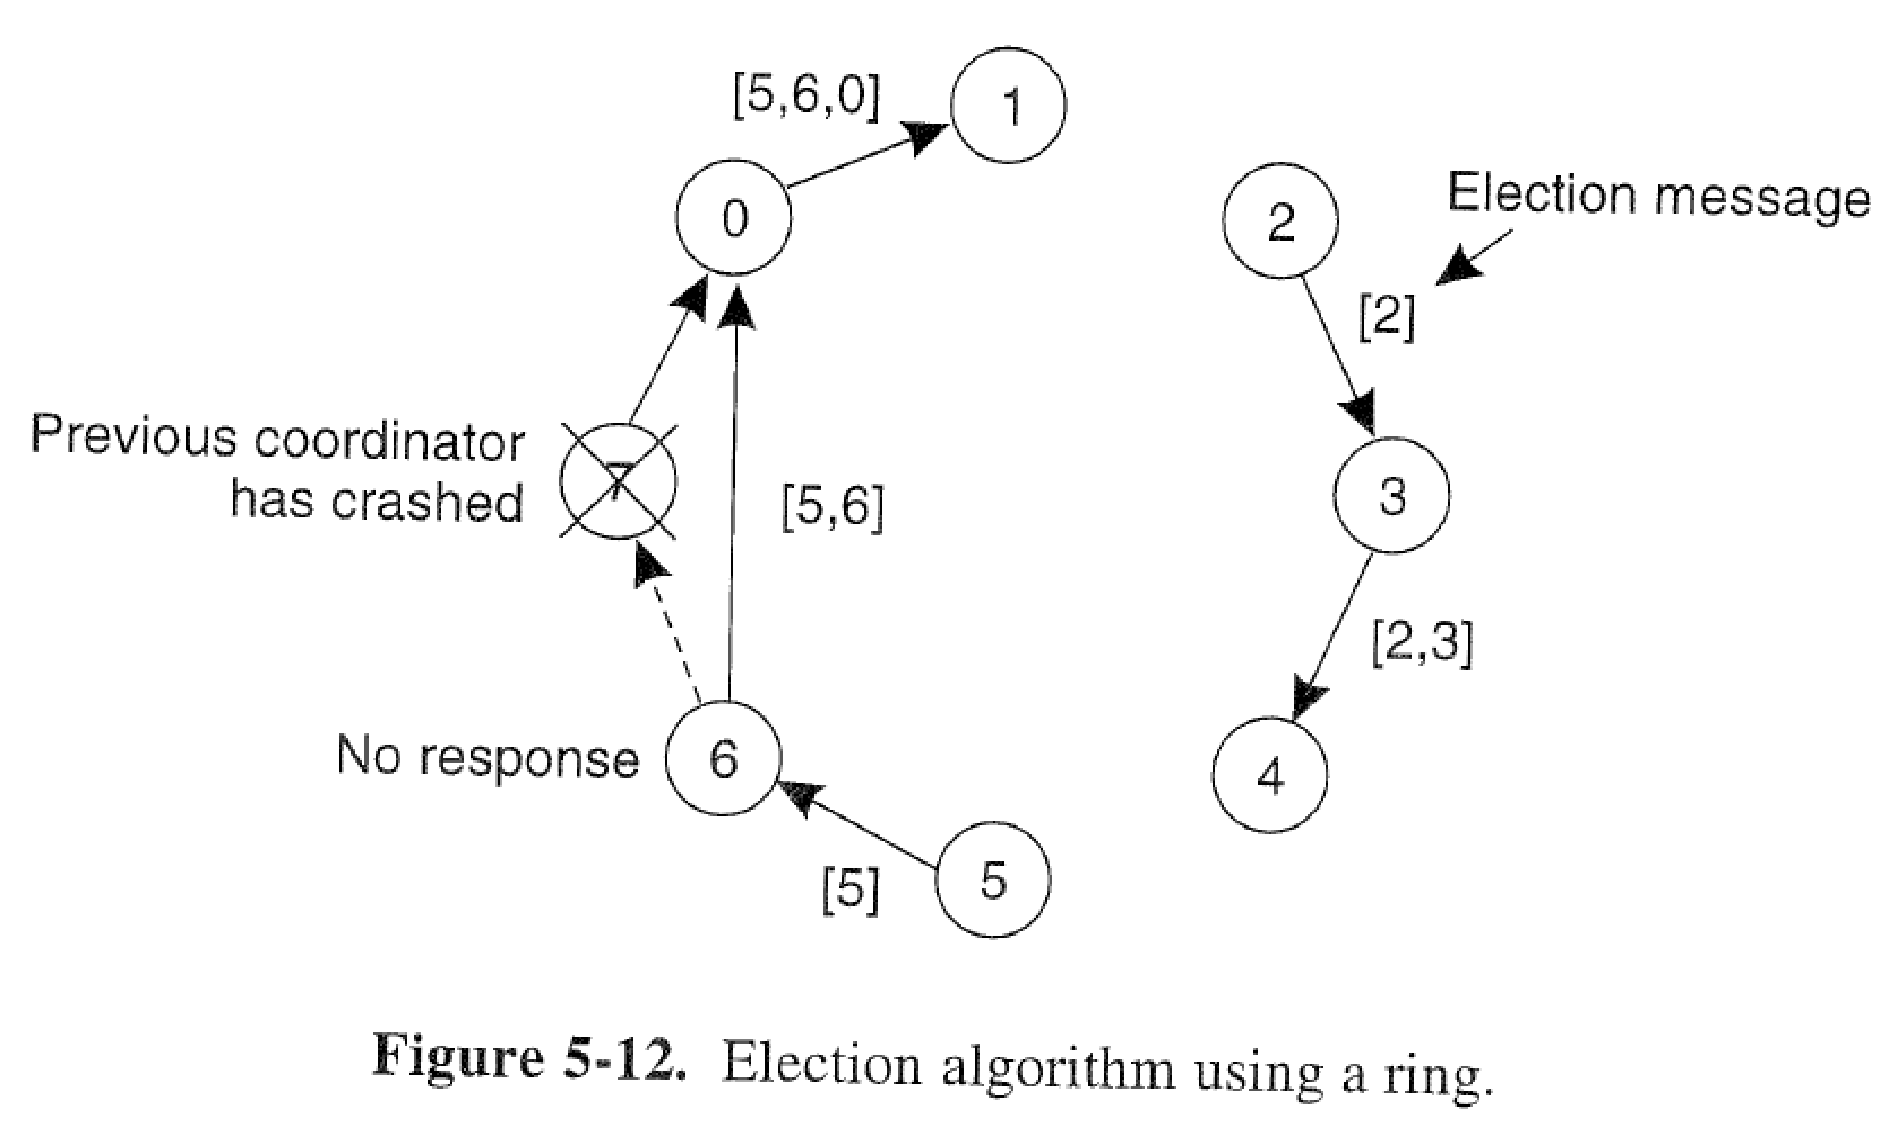
\includegraphics[width=1\linewidth]{example_ring.pdf}
    \caption{Příklad činnosti Ring algoritmu.}
\end{figure}

%%%%%%%%%%%%%%%%%%%%%%%%%%%%%%%%%%%%%%%%%%%%%%%%%%%%%%%%%%%%%%%%%%%%%%%%%%%%%%%%

\section{Algoritmus pro obecnou topologii}

Předpokládáme, že nemáme ani kruhovou topologii ani spojení každý s~každým. Např.: peer-to-peer sítě, sensorové sítě, \dots

\subsection{Postup}

\begin{compactitem}
    \item V~první iteraci se broadcastem posílá zpráva ELECTION.
    \item Každý uzel si uloží od kterého souseda dostal zprávu ELECTION jako první. Tím vzníká kostra grafu (\textit{spanning tree}).
    \item Uložený soused je poté využijí pro zpětnou komunikaci. To znamená, že další komunikace už probíhá přes strom, nikoliv přes broadcast. Tím je ušetřena některé komunikace.
\end{compactitem}

\subsection{Složitost}

Složitost z~hlediska počtu zpráv.

\begin{compactitem}
    \item Inicializační broadcast: počet hran grafu.
    \item Odpověď: počet hran kostry grafu.
    \item Result broadcast: počet hran kostry grafu.
\end{compactitem}

\subsection{Příklad}

\begin{figure}[H]
    \centering
    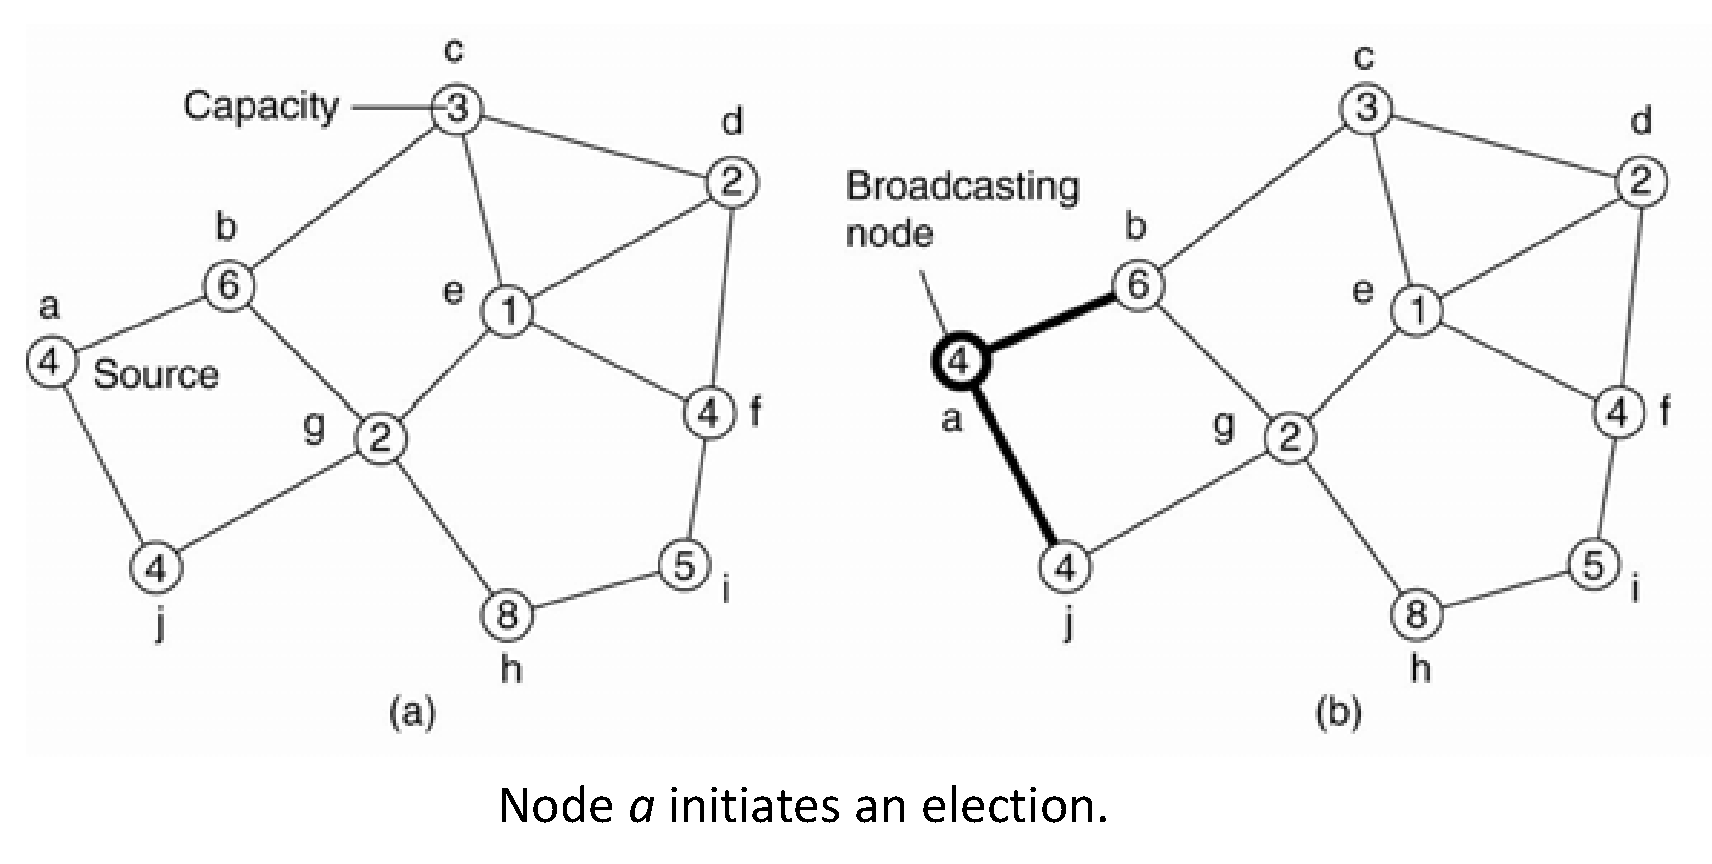
\includegraphics[width=1\linewidth]{example_general_topology_p1.pdf}
    \caption{Příklad činnosti algoritmu pro obecnou topologii, část 1.}
\end{figure}

\begin{figure}[H]
    \centering
    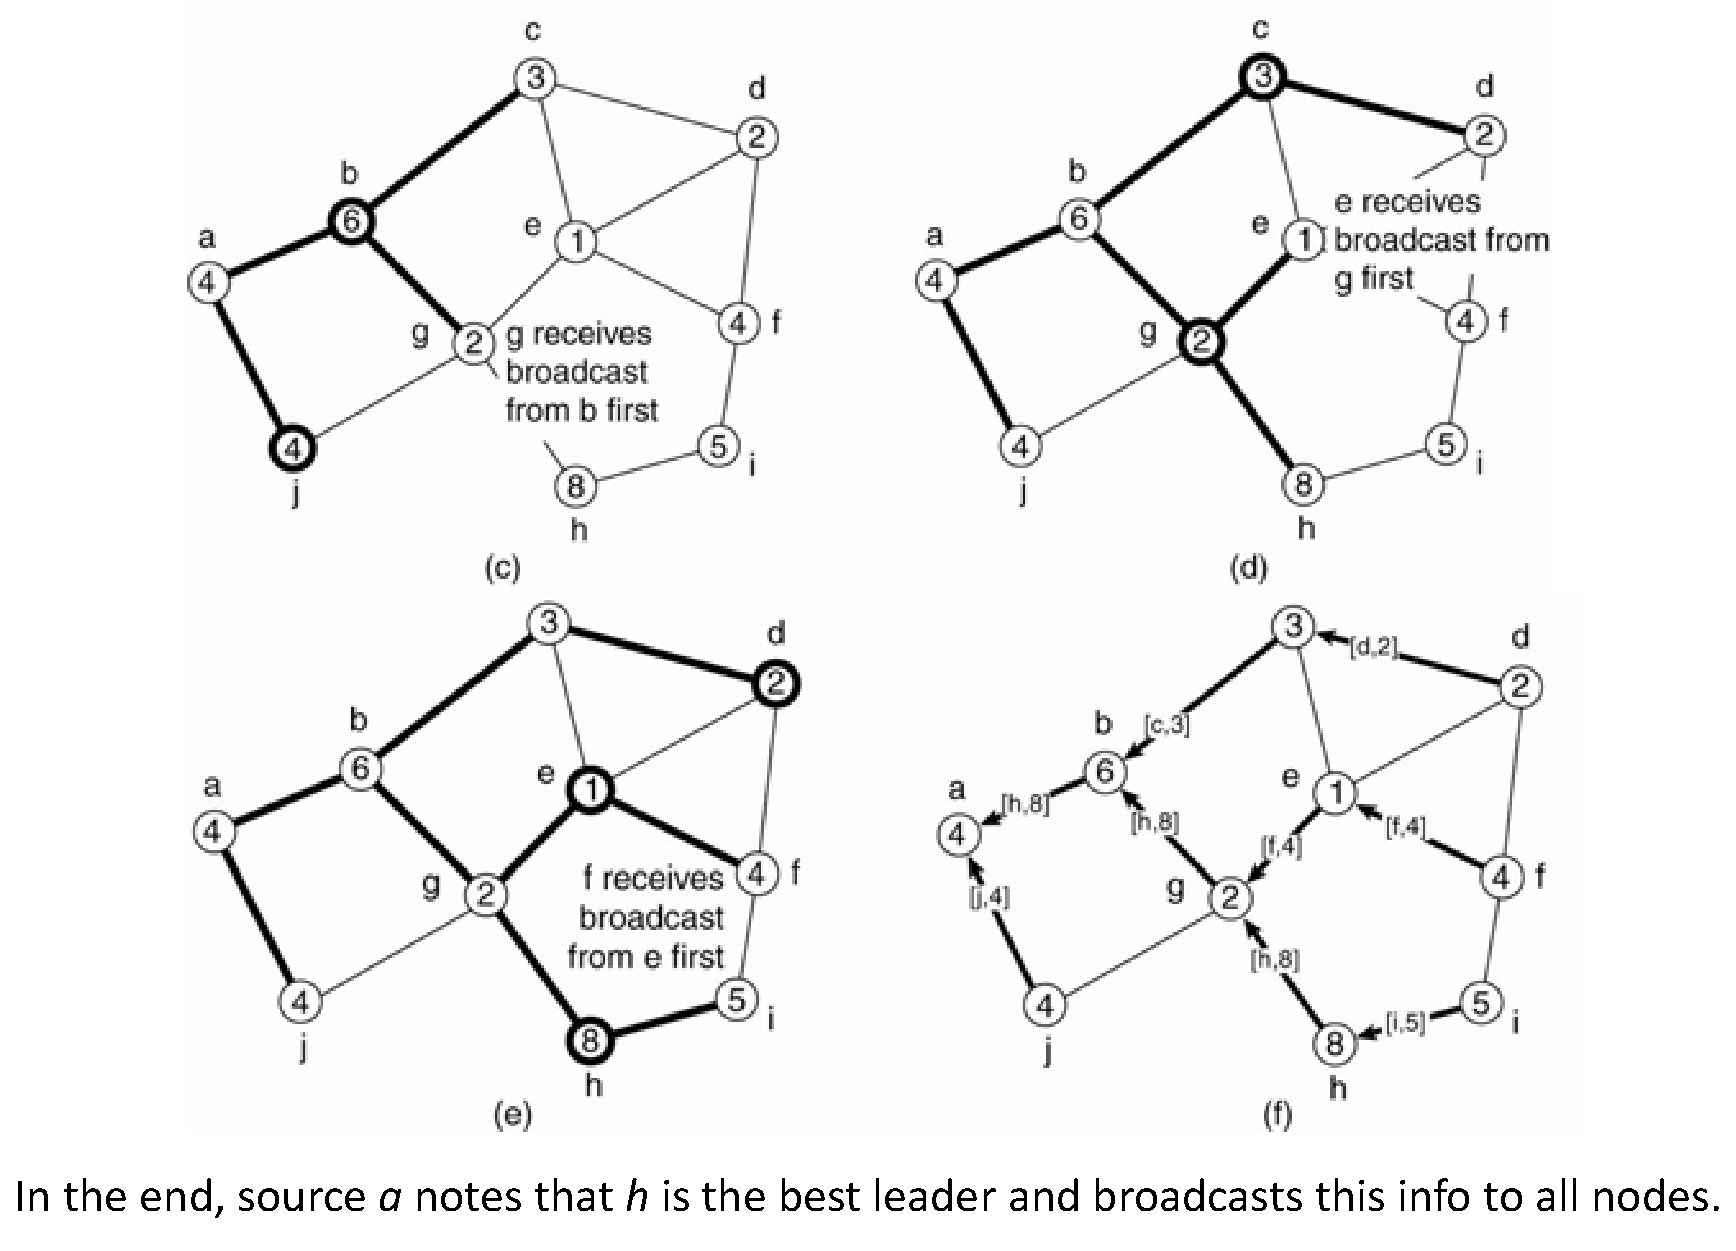
\includegraphics[width=1\linewidth]{example_general_topology_p2.pdf}
    \caption{Příklad činnosti algoritmu pro obecnou topologii, část 2.}
\end{figure}
